\chapter{Dataset HAM10000}
\label{cap:nomePrimoCapitoloTesi}
\lhead{\textbf{\rightmark}}
In questa sezione è stato descritto il dataset utilizzato per addestrare la rete neurale convoluzionale.

\section{Introduzione al Dataset}
\label{sec:nomePrimaSezioneCapitolo}

\indent{
	Il dataset HAM10000 (Human Against Machine con 10000 immagini di addestramento) è stato utilizzato in questo progetto come dataset di addestramento.
	\footnote{Il dataset HAM10000 è disponibile su Kaggle. https://www.kaggle.com/kmader/skin-cancer-mnist-ham10000/kernels} \cite{kaggle}
	Questo dataset contiene lesioni cutanee pigmentate acquisite mediante un dematoscopio standard.
	\begin{figure}[h]
		\begin{center}     
			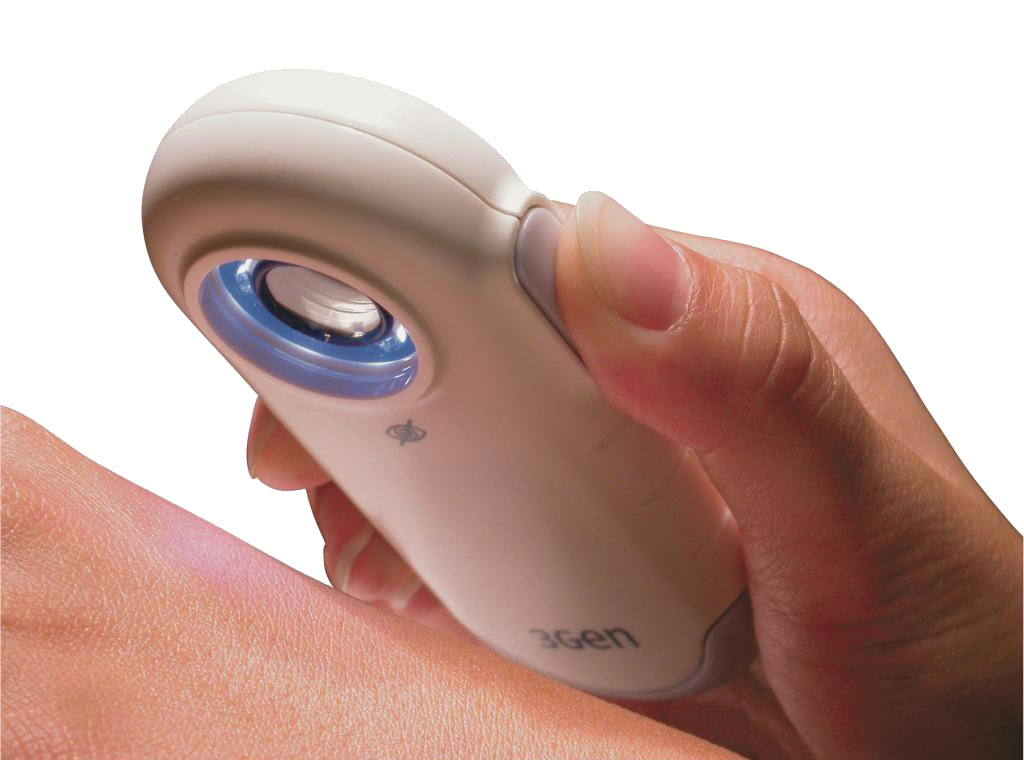
\includegraphics[scale=0.20]{figure/capitolo2/dermatoscopio.jpg}
		\end{center}
		\caption{Esempio di un dermatoscopio}	
	\end{figure}
	\newline
	\newline
	Non tutti i tipi di lesioni inizialmente studiati e sottoposti a triage attraverso la dermatoscopia sono necessariamente lesioni pigmentate. Ciò significa che, in una situazione del mondo reale, un medico generico o un infermiere che esaminano un paziente attraverso la dermatoscopia (o un paziente che esegue l'autoesame) con l'intento di presentare queste immagini a un dermatologo per un triage iniziale, potrebbero incontrare altre lesioni rispetto a quelli raffigurati in questo dataset.
	\newline
	Le lesioni classificate nel dataset HAM10000 sono: \cite{tschandl2018ham10000}
	\begin{enumerate}
		\item nv: Melanocytic nevi - neoplasie benigne dei melanociti [6705 immagini];
		\item mel: Melanoma - una neoplasia maligna derivata dai melanociti [1113 immagini]
		\item 	bkl: Cheratosi benigna - una classe generica che comprende cheratosi seborroiche, lentigo solare e lichen-planus come cheratosi [1099 immagini];
		\item cc: carcinoma basocellulare - una variante comune del carcinoma epiteliale della pelle che raramente metastatizza ma cresce in modo distruttivo se non trattata (le cc non producono necessariamente lesioni pigmentate) [514 immagini];
		\item akiec: cheratosi attinica e carcinoma intraepiteliale - varianti non invasive comuni del carcinoma a cellule squamose che possono essere trattate localmente senza chirurgia [327 immagini];
		\item vasc: lesioni cutanee vascolari che vanno dagli angiomi di ciliegia agli angiocheratomi e ai granulomi piogeni [142 immagini];
		\item df: dermatofibroma - una lesione cutanea benigna considerata come una proliferazione benigna o una reazione infiammatoria a un trauma minimo [115 immagini].
	\end{enumerate}
	
	\section{Limiti diagnostici di questo dataset}
	Le immagini dermatoscopiche da sole non forniscono dati sufficienti per una diagnosi dermatologica o un triage remoto affidabile del paziente in un ambiente di Teledermatologia.\cite{tschandl2018ham10000}
	\newline
	Le immagini dermatoscopiche mancano di contesto. Al fine di fornire un contesto, sarà necessario eseguire un protocollo di acquisizione delle immagini che includa immagini panoramiche di tutto il corpo del paziente e anche immagini di approssimazione di ciascuna lesione, che vengono acquisite con un righello o un altro quadro di riferimento visibile nell'immagine, al fine di fornire informazioni contestuali sulla dimensione della lesione. 
	\newline
	Le immagini di approssimazione scattate con il righello sono importanti anche per un paziente già in trattamento per consentire al medico assegnato di seguire l'evoluzione della lesione. Sia le immagini panoramiche che quelle di approssimazione, per essere acquisite correttamente, devono essere eseguite seguendo un protocollo che garantisca che le immagini siano a fuoco (nitide e non sfocate), prese dalla distanza corretta e con l'illuminazione corretta. \cite{von2019creating}
	Vi sono anche dettagli che non possono essere rilevati in modo affidabile attraverso la tecnica standard di dermatoscopia attualmente in uso e, in diversi casi, sarà necessaria una biopsia di conferma (noto anche come esame istologico).
	\footnote{Per un maggiore approfondimento sui protocolli di acquisizione degli esami di Teledermatologia: Aldo von Wangenheim and Daniel Holthausen Nunes. Creating a Web Infrastructure for the Support of Clinical Protocols and Clinical Management: An Example in Teledermatology. Telemedicine and e-Health. Online Ahead of Print:November 30, 2018. http://doi.org/10.1089/tmj.2018.0197. There’s also a preprint available on ResearchGate.}
	
	\section{Acquisizione immagini dermoscopiche}
	Il dermoscopio a contatto utilizzato al giorno d'oggi è il risultato di uno sforzo internazionale per la standardizzazione di questo esame effettuato durante la prima metà degli anni '90, guidato da un gruppo di ricercatori dell'Università di Monaco in Germania. Questa apparecchiatura utilizza una singola lente con un ingrandimento di 10x e un'illuminazione interna tramite LED. L'esame viene eseguito con olio minerale, che viene applicato sulla superficie della lesione prima che il dermoscopio venga applicato sulla lesione e venga scattata una fotografia.
	\begin{figure}[h]
		\begin{center}     
			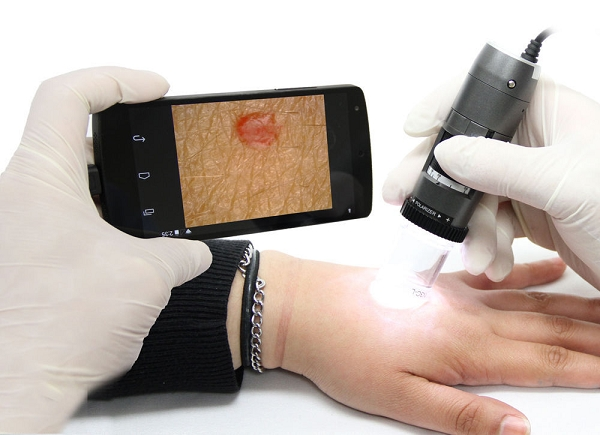
\includegraphics[scale=0.30]{figure/capitolo2/dermatoscopio.png}
		\end{center}
		\caption{Esempio a scopo illustrativo di un dermatoscopio digitale}	
	\end{figure}
	La scelta di una lente di ingrandimento monoculare 10x come standard ha consentito lo sviluppo di dispositivi molto piccoli che presto sono diventati molto popolari.
	\newline
	I dermoscopi analogici possono essere trasportati in un taschino e quelli digitali possono essere facilmente sviluppati come piccoli dispositivi USB o come adattatori per fotocamere digitali e smartphone.
	\newline
	Lo svantaggio di questo standard è che l'ingrandimento 10x non è sufficiente per il rilevamento affidabile di alcune patologie, come il carcinoma a cellule basali, che è la forma più comune di cancro della pelle. 
	\newline
	Questa forma di neoplasia è caratterizzata da alterazioni vascolari, chiamate vascolarizzazioni arboriformi, che non possono essere osservate in modo affidabile con una lente monoculare che impiega un ingrandimento 10x: sarà sempre necessaria una biopsia di conferma al fine di fornire la diagnosi definitiva.
	\newline
	Il rilevamento affidabile richiede un ingrandimento maggiore e un'ottica binoculare.
	\cite{rajpara2009systematic}

}
